
\documentclass[a4paper,12pt]{article}
\usepackage[utf8]{inputenc}
\usepackage[spanish,es-nodecimaldot]{babel}
\usepackage[T1]{fontenc}
\usepackage[intlimits]{amsmath}
\usepackage{graphicx}
\usepackage{a4wide}
\usepackage{float}
\usepackage{verbatim}
\usepackage[labelfont={bf},textfont={it}]{caption}
\usepackage{subcaption}


\usepackage{hyperref}
\hypersetup{ %
colorlinks=false  % false:boxedlinks ; true:coloredlinks
} %


\usepackage{tikz}
\usetikzlibrary{trees}
\usepackage{xcolor}

\graphicspath{{imagenes/}}

\title{\textsc{Dinámica Molecular} \\ \vspace{2em} \Large{Introducción a la 
simulación computacional}}
\author{\small{ Pablo Bellino (pbellino@gmail.com)} \\
        \small{Luis María Pizarro (lpizarro@cnea.gov.ar)}}

\date{Noviembre de 2015}


\begin{document}

%\inputencoding{latin1}

\maketitle

\begin{abstract}
Se implementó el algoritmo de dinámica molecular con el objeto de estudiar un 
sistema de partículas que interactúan a través de un potencial de 
Lennard-Jones. Se estudió el comportamiento bulk del sistema para distintos 
puntos del espacio de fases y cómo varian sus propiedades termodinámicas en las 
zonas de transición. Se trabajó en el ensamble canónico por medio del 
termostato de Langevin. Se obtuvieron las funciones de correlación entre 
pares para algunas configuraciones típicas.
\end{abstract}


\section{Introducción}

En este trabajo se aplicó el método de dinámica molecular para estudiar el 
comportamiento termodinámico de un sistema de partículas interactuantes de a 
pares por medio de un potencial de Lennard-Jones.

Este sistema de líquido de Lennard-Jonnes es ampliamente utilizado para 
estudiar el comportamiento de fluidos simples y como base para teorías 
perturbativas de fluídos más complejos.

El método consistió en resolver las ecuaciones de Newton para un Hamiltoniano 
de la forma:

\begin{equation}\label{eq:hamiltoniano}
  \mathcal H({\bf r},{\bf p}) = \sum_{i=1}^{N} \frac{p_i^2}{2m} + \sum_{i=1}^N \sum_{j>i} \phi (r_{ij})
\end{equation}

\noindent en donde se utilizó el potencial de interacción entre pares de 
Lennard-Jones:

\begin{equation}\label{eq:pot_LJ}
  \phi (r) = 4\epsilon\left[\left(\frac{\sigma}{r}\right)^{12} -\left(\frac{\sigma}{r}\right)^{6}\right]
\end{equation}

Se estudiaron distintas configuraciones del espacio de fases del sistema. En 
cada caso, se efectuaron varias corridas para obtener un análisis estadístico 
adecuado. Se trabajó en el ensamble canónico utilizando el termostato de 
Langevin para fijar la temperatura. 

\section{Implementación del método}

Para evitar trabajar con interacciones entre todas las partículas, se utilizó 
el método del potencial truncado y desplazado definido como:

\begin{equation}\label{eq:pot_cs}
  \phi_{cs}(r) = 
  \begin{cases}
	  \phi(r)- \phi(r_c) \quad \text{si } r \leq r_c \\
	  0 \hspace{2.4cm} \text{si } r > r_c
  \end{cases}
\end{equation}

\noindent en donde $r_c$ es el radio de corte más allá del cual se considera 
que no existe interacción alguna. En este trabajo se utilizó un valor de 
$r_c=4\sigma$. Dicho valor fue elegido para comparar más adecuadamente los 
valores de referencia dados por \cite{johnson1993}.

Como es usual, se utilizaron unidades reducidas en donde la dinstancia y la 
energía se miden en unidades de $\sigma$ y $\epsilon$, del potencial de LJ; y 
la masa en unidades de masa de partícula. El resto de las magnitudes se 
derivan a partir de estas tres. En el Cuadro \eqref{tb:unidades} se dan las 
unidades reducidas de las principales magnitudes utilizadas.

\begin{table}
	\begin{center}
		\begin{tabular}{ccc}
			\hline
			{\bf Magnitud} & {\bf Símbolo} & {\bf Unidad} \\ \hline
			Distancia   & $L^*$ & $\sigma$ \\ 
			Energía     & $E^*$ & $\epsilon$ \\ 
			Masa        & $m^*$ & $m$ \\ 
			Tiempo      & $t^*$ & $\sigma\sqrt{m/\epsilon}$ \\ 
			Temperatura & $T^*$ & $k_b/\epsilon$ \\ 
			Presión     & $p^*$ & $\epsilon/\sigma^3$ \\ 
			Fuerza      & $F^*$ & $\epsilon/\sigma$ \\ 
			\hline 
		\end{tabular}
	\end{center} 
	\caption{Unidades reducidas utilizadas en la simulación}
	\label{tb:unidades}
\end{table}

El sistema simulado consistió en un cubo de lado $L$ con una cantidad de 
partículas de $N_{part}=200$. Como se pretendía estudiar el bulk, se tomaron 
condiciones periódicas de contorno en todas sus caras. Se utilizó el método de 
mínima imágen para garantizar que se estuviera contando sólo una interacción 
por cada partícula o imagen. 

La integración de las ecuaciones de Newton se realizó con el algoritmo de 
Velocity-Verlet, con un paso temporal de integración de $dt=0.001$.

\subsection{Termostato de Langevin}

Para poder trabajar en el ensamble canónico a una temperatura fija fue 
necesario implementar un termostato que obligara al sistema a intercambiar 
energía y de esta manera establecer la temperatura de trabajo. De lo contrario, 
se estaría trabajando en el ensamble micro-canónico a energía constante.

El termostato implementado fue el de Langevin, que consiste en aplicarle a cada 
partícula una fuerza aleatoria dada por la expresión (en unidades reducidas):

\begin{equation}\label{eq:termo}
 F_i^{\it lang} = - \gamma  v_i + \sqrt{\frac{2\gamma T}{\Delta t}} \mathcal 
 N(0,1)
\end{equation}

\noindent donde $\mathcal N(0,1)$ es una distribución normal estándar (media 
nula y desviación estandar unidad). Se utilizó un valor de $\gamma=0.5$ a lo 
largo de todo el trabajo.

Se mostrará en la parte de resultados un método para corroborar el buen 
funcionamiento del termostato de Langevin.

\subsection{Mediciones}

Las dos magnitudes medidas de mayor importancia durante la simulación fueron la 
presión instantánea y la temperatura instantánea. De ambas mediciones, luego 
fue posible tomar un valor medio y encontrar la presión y temperatura 
termodinámicas que intervienen en la ecuación de estado.

La temperatura instantánea fue medida utilizando su relación estadística con la 
energía cinética del sistema. Su definición se expresa como:

\begin{equation}\label{eq:tempe}
 T(t) = \frac{1}{3N-3} \sum_{i=1}^{N} m {\bf v_i}^2
\end{equation}

Por otro lado, la medición de la presión se realizó utilizando el teorema del 
Virial. En este caso, y por tener un potencial que sólo depende de la distancia 
entre partículas, la presión puede escribirse como:

\begin{equation}\label{eq:pres}
p(t) = \rho T  - \frac{1}{3V} \sum_{i=1}^N \sum_{j>i} r_{ij} \frac{\phi(r_{ij})}{dr}
\end{equation}

\noindent en donde $V=L^3$ es el volumen del sistma. El primer término 
corresponde a la presión que tendría un gas ideal y el segundo es que proviene 
de la interacción entre las partículas. En el primer término se utilizó la 
temperatura instantánea medida en vez de la temperatura fija de entrada.

El término del virial fue calculado dentro del loop de fuerzas para evitar 
tener que realizar un segundo doble loop sobre todas las interacciones.

Finalmente, también se registraron los valores de otras magnitudes de interés, 
como la energía interna del sistema, la energía total y las posiciones de las 
partículas. Algunas de estas magnitudes por no ser relevantes para todos los 
análisis, fueron activadas o desactivadas con el preprocesador para no lentizar 
los tiempos de corrida del programa.

\section{Resultados}

En esta sección se muestran los resultados obtenidos durante las distintas 
corridas del programa. Para facilitzar su análisis se dividieron los resultados 
en dos partes. En la primer parte se realizó un barrido de temperaturas 
dejando la densidad de partículas fija, mientras que en la segunda se hizo un 
barrido de densidad a una temperatura fija.

En la Figura \eqref{fig:fases} se muestran esquemáticamente (en rojo) ambos 
barridos sobre el diagrama de fases del sistema de Lennard-Jones. Esta figura 
permitirá, a su vez, analizar los resultados obtenidos dependiendo en qué parte 
del diagrama se realizó cada simulación.

\begin{figure}[H]
	\centering
	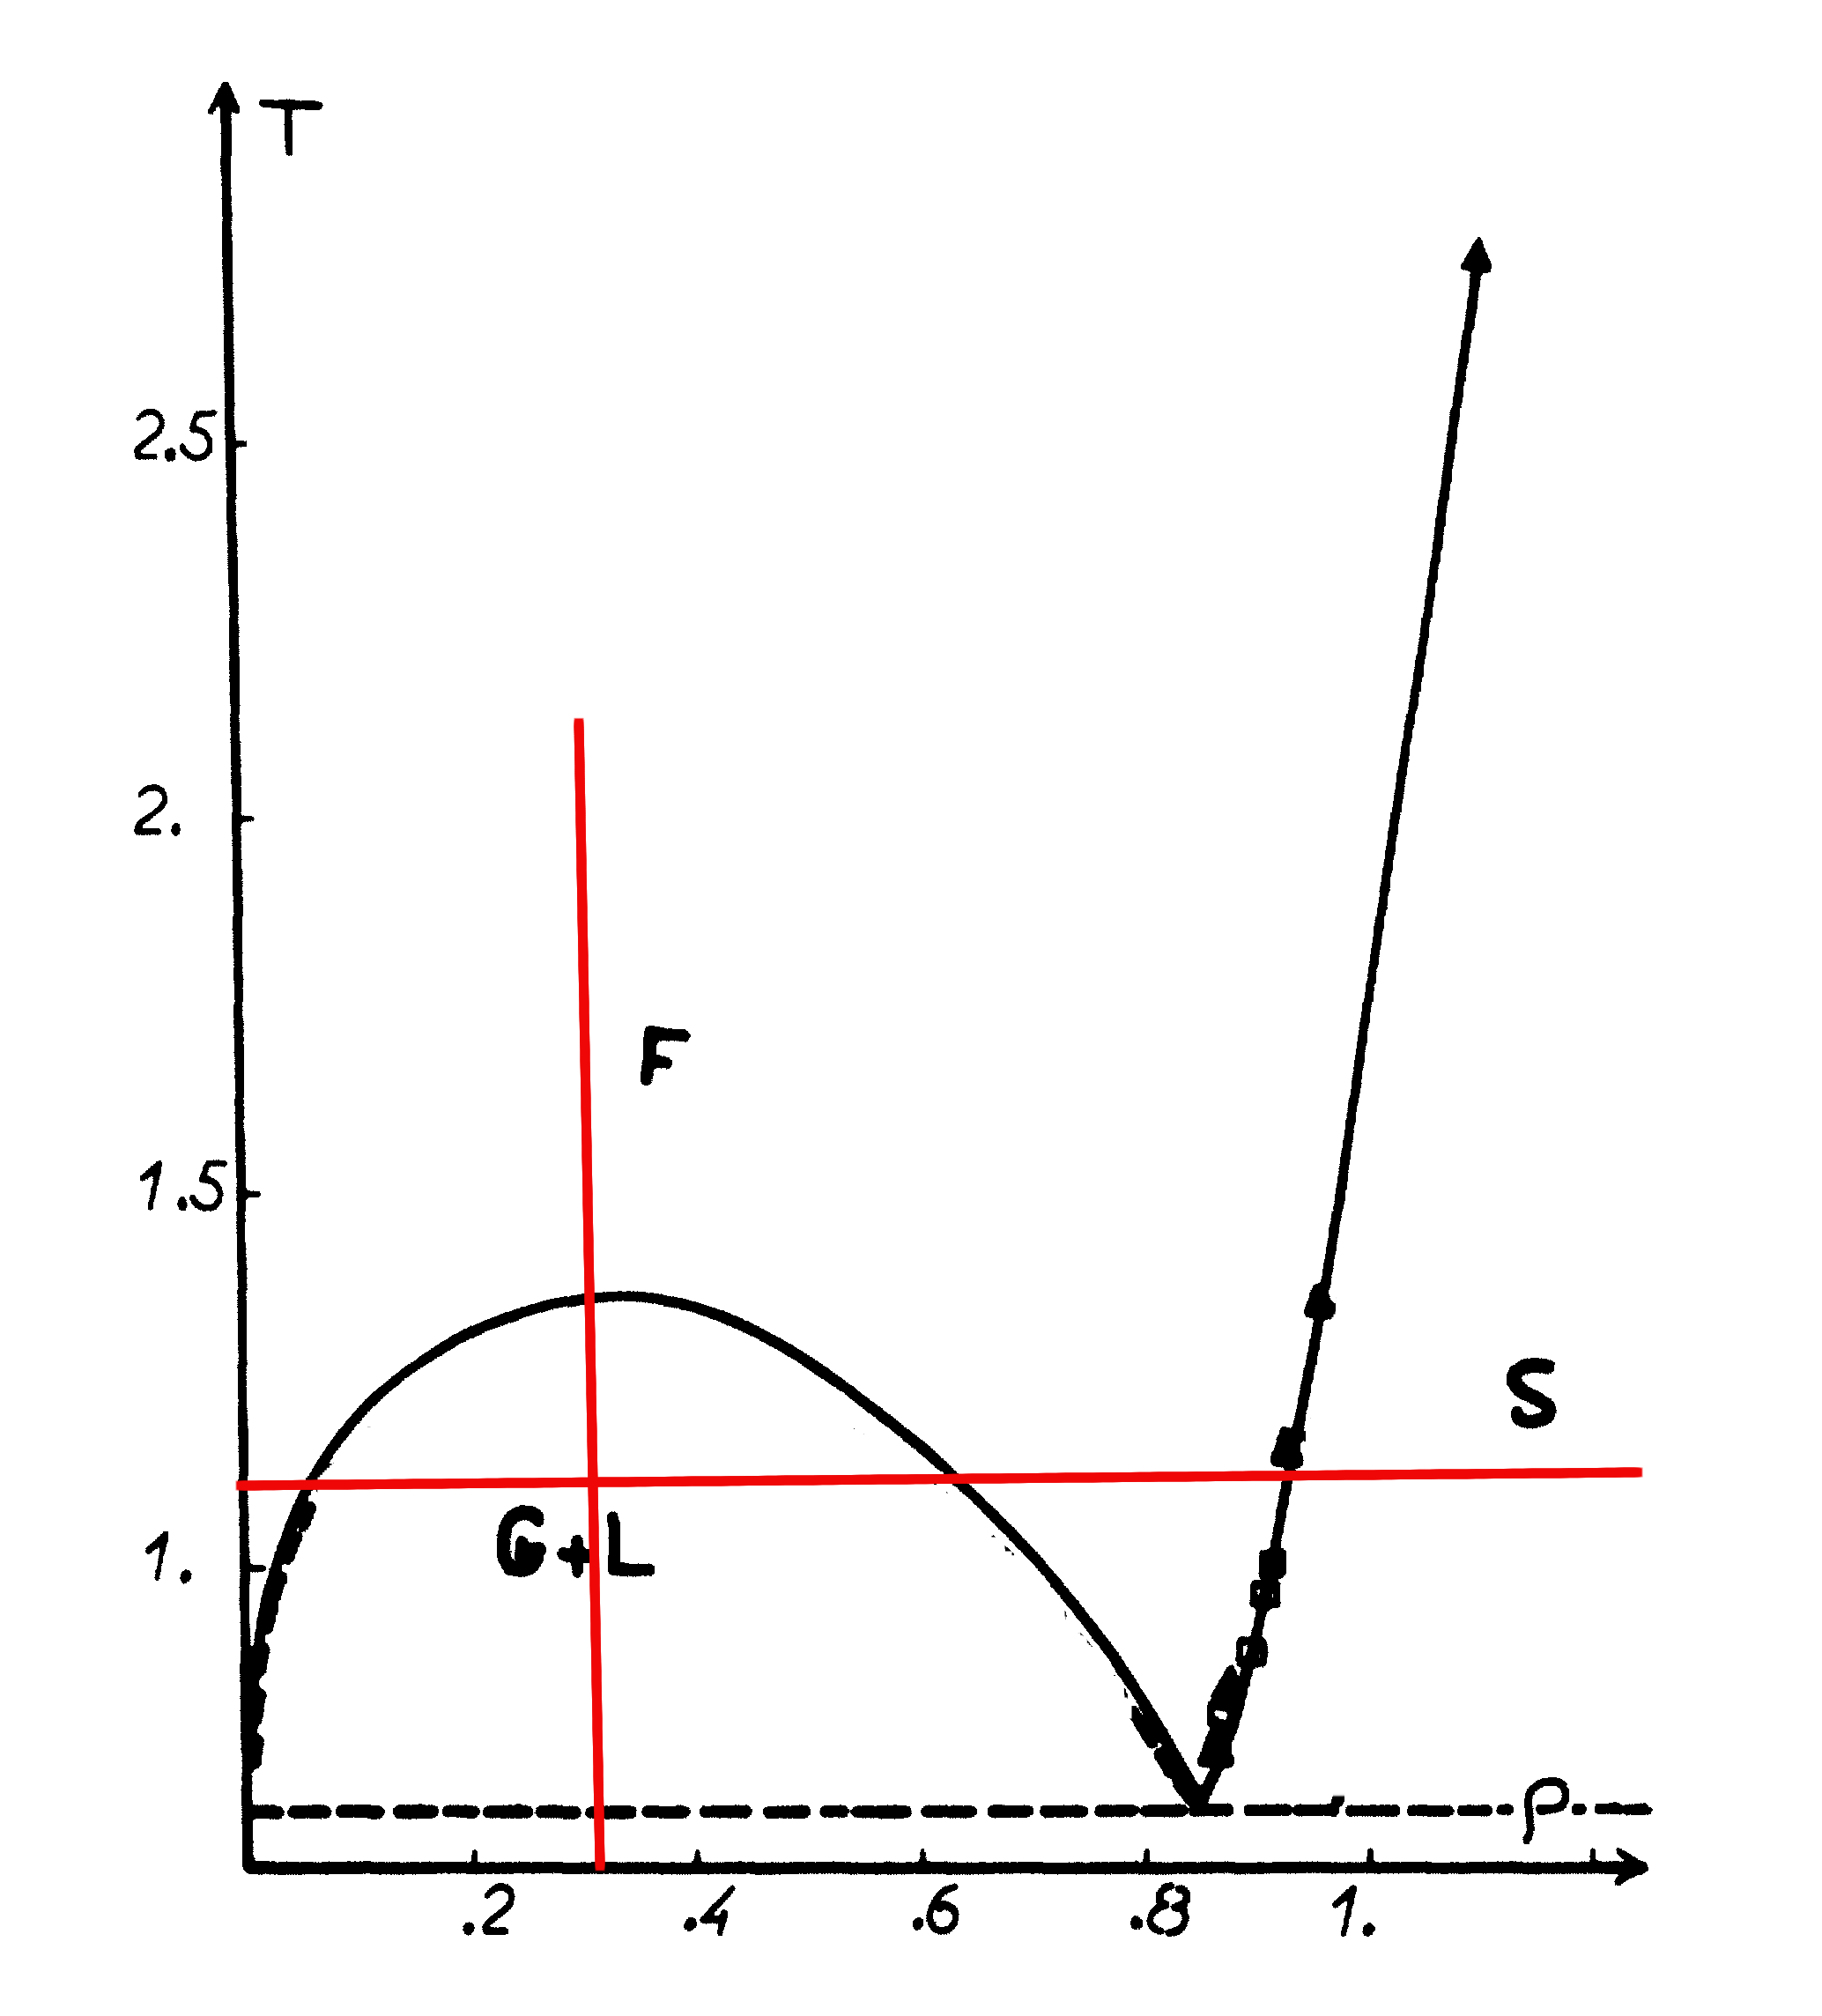
\includegraphics[scale=0.13]{fases.png} \\
	\caption{Diagrama de fases del sistema de Lennard-Jones junto con las 
	indicaciones sobre los distintos estados simulados (en rojo). Gráfico 
	original extraido de \cite{hansenverlet1969}}\label{fig:fases}
\end{figure}

\subsection{Verificación del termostato de Langevin}

Antes de realizar el estudio sistemático variando los parámetros, se realizó 
una comprobacióń para verificar que el termostato de Langevin estuviese bien 
implementado.

La primera validación se realizó analizando el gráfico de la temperatura en 
función del tiempo para el sistema en equilibrio. Se realizó una corrida con 
$\rho^*=0.8$ y $T^*=1.0$. En la Figura \eqref{fig:termo_tempe} se muestra el 
resultado obtenido.

\begin{figure}[H]
	\centering
	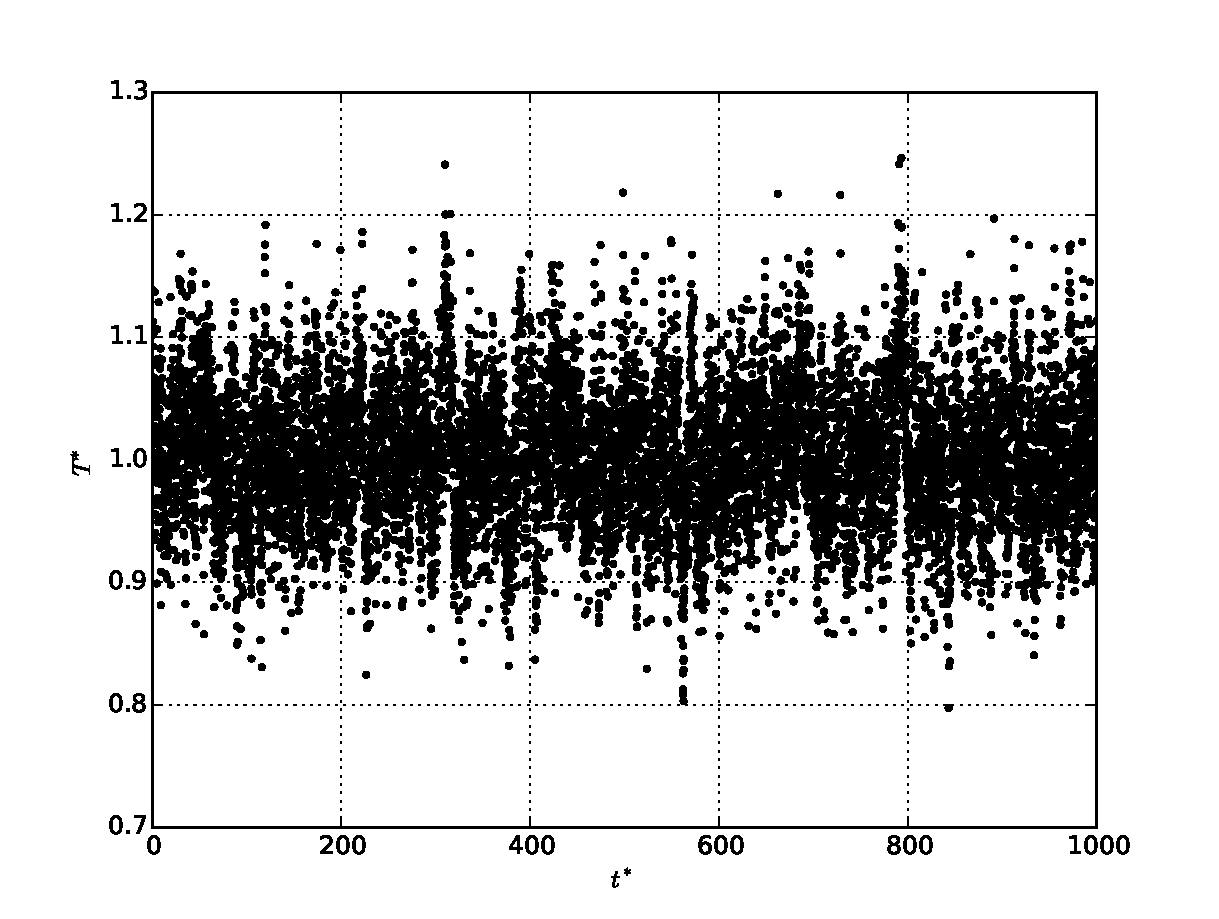
\includegraphics[scale=0.5]{termo_tempe.pdf} \\
	\caption{Temperatura instantánea en función del tiempo para $T^*=1.0$ 
	utilizando el termostato de Langevin}\label{fig:termo_tempe}
\end{figure}

El comportamiento de la temperatura es el esperado, con un valor medio 
alrededor del valor fijado de temperatura y una fluctuación debida a la 
característica propia del termostato.

Es posible, sin embargo, realizar una validación más detallada analizando si la 
fluctuaciones obtenidas son las que corresponden con la física del problema. En 
particular, se analizó la fluctuación de la componente de velocidad de una 
partícula arbitraria a lo largo de una simulación.

Para un sistema en quilibrio en el ensamble canónico, es posible demostrar que 
el módulo cuadrado de la velocidad tiene una distribución de Maxwell-Boltzmann, 
de lo cual se deduce que cada componente de la velocidad posee una distribución 
Gaussiana dada por:

\begin{equation}\label{eq:dist_gauss}
f (v_i) =
\sqrt{\frac{m}{2 \pi k_bT}} \exp \left[ \frac{-mv_i^2}{2k_bT} \right]
\end{equation}

\noindent de donde se desprende que la varianza de dicha distribución será (en 
unidades reducidas):

\begin{equation}\label{eq:termo_sigma}
\sigma^2(v^*_i) = T^*
\end{equation}

Para implementar esta validación, se eligió arbitrariamente una partícula, y se 
registró una componente arbitraria de su velocidad a lo largo de toda la 
simulación. Se realizó el histograma correspondiente y se ajusaron los datos 
obtenidos con una función Gaussiana. En la Figura \eqref{fig:termo_histo} se 
muestran los resultados obtenidos. Se omitió la normalización del histograma ya 
que no era relevante para el presente análisis.

\begin{figure}[H]
  \centering
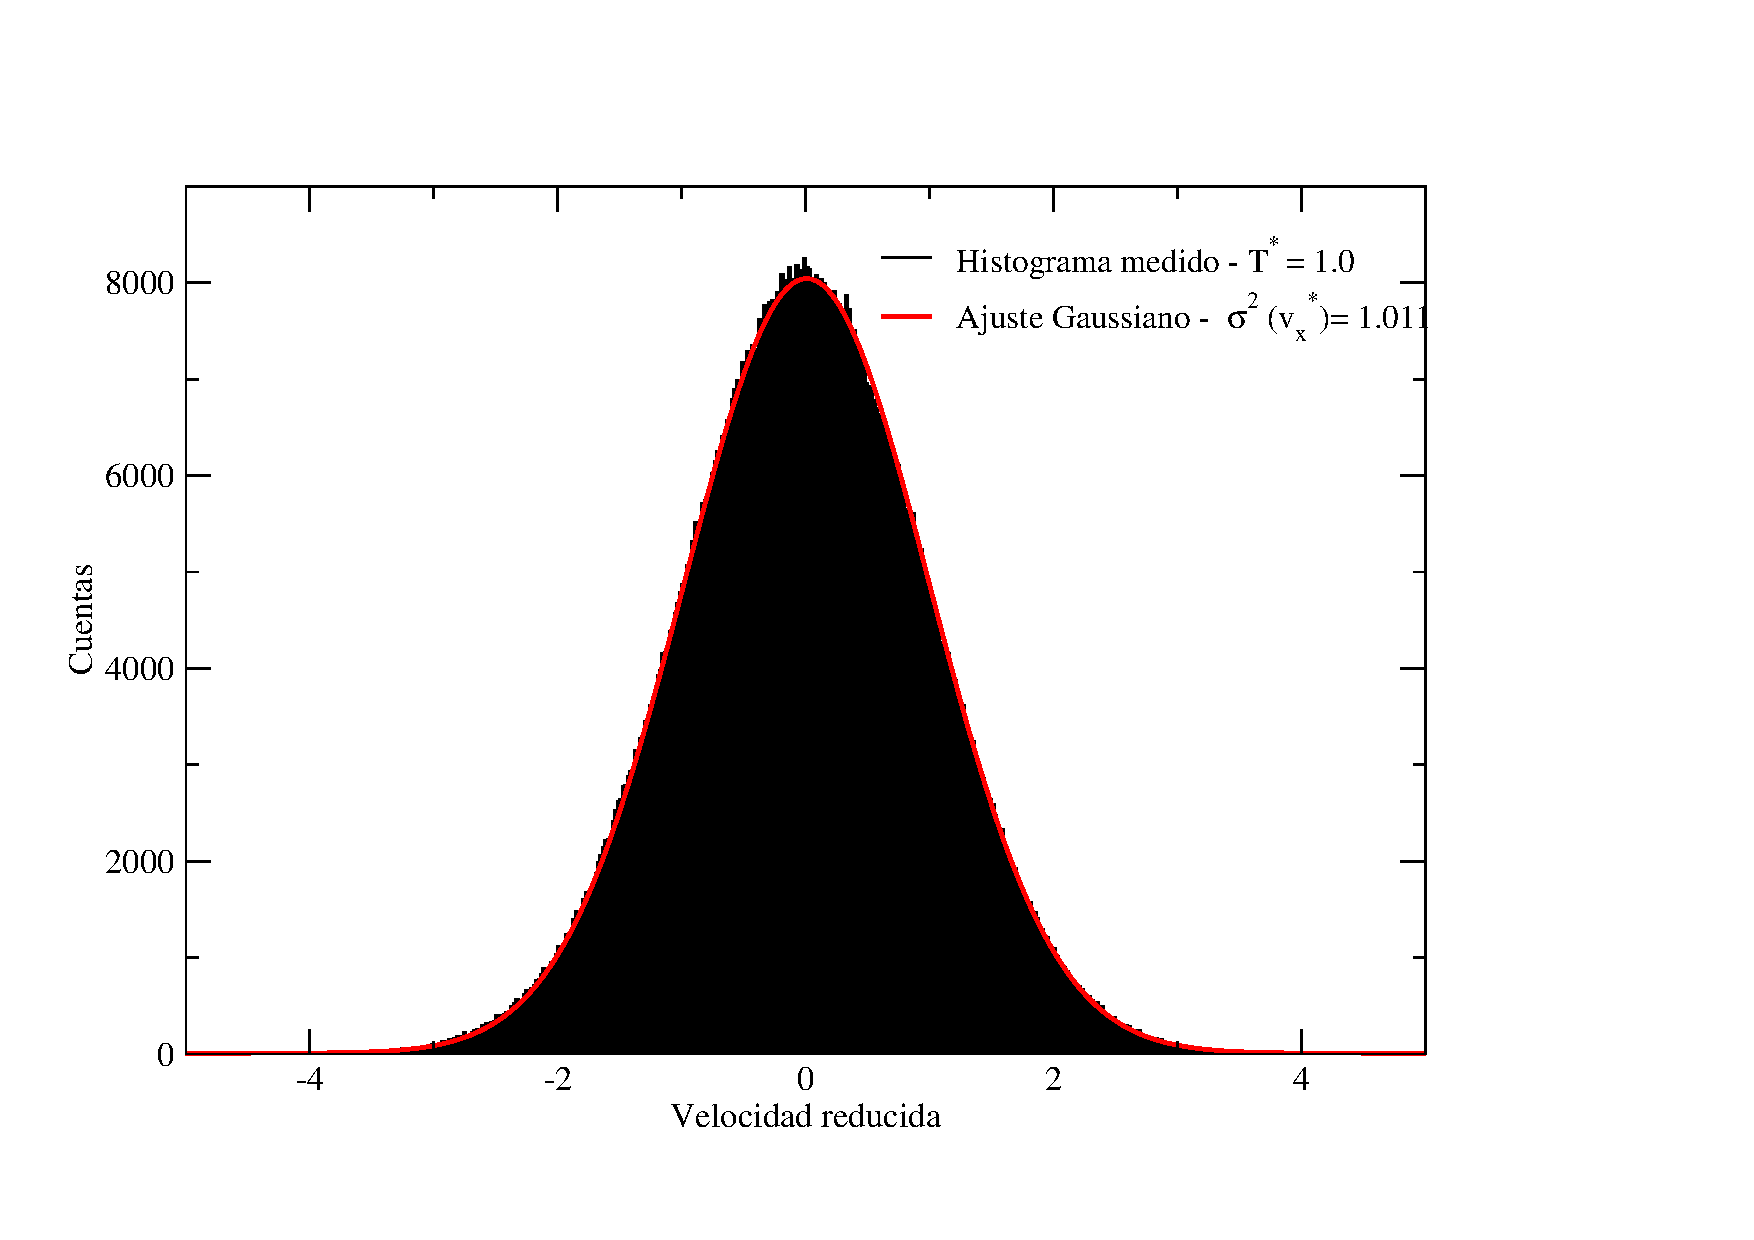
\includegraphics[scale=0.6]{termo_histograma.pdf} \\
\vspace{-2em}
\caption{Histograma de la componente de velocidad de una partícula con el 
correspondiente ajuste Gaussiano para $T^*=1.0$.}\label{fig:termo_histo}
\end{figure}

La distribución de velocidades obtenida concuerda a simple vista con una 
distribución Gaussiana. La varianza estimada a partír del ajuste fue de 
$\sigma^2(v_x^*) = 1.011$. Los resultados encontrados con este análisis 
permiten indicar que la implementación del termostato de Langevin es correcta.
	

\subsection{Barrido de temperatura a densidad constante}

En este punto se muestran los resultados obtenidos al realizar distintas 
corridas dejando la densidad constante en $\rho^*=0.3$ y cambiando la 
temperatura en el rango $[0.7\, , \, 1.4]$ con pasos de $dT=0.05$. Los 
parámetros utilizados para esta simulación fueron $N_{med} = 5\,10^6$, 
$N_{run} = 20$ corridas para cada configuración. El resto de los parámetros 
tuvieron valores similares a los descriptos anteriormente.

En la Figura \eqref{fig:temp} se muestran los resultados más relevantes de 
estas simulaciones. En la Figura \eqref{fig:temp_p} se realiza el gráfico de 
los valores medios de la presión para cada temperatura. Los valores de 
temperatura graficados fueron los obtenidos a través de las mediciones (no del 
valor fijado como entrada), con sus 
respectivos errores.

Se compararon los resultados obtenidos con los valores de referencia en 
\cite{johnson1993} obteniéndose similares valores (no todos estaban 
disponibles en las tablas de referencia, se interpolaron puntos cuando fue 
necesario). Se tuvo la precaución de utilizar el mismo radio de corte ($r_c = 4 
\sigma$) para que la comparación sea válida, sin embargo la cantidad de 
particulas utilzada en la referencia fue de $864$ mientras que la del presente 
trabajo fue de $200$.

\begin{figure}[H]
	\centering
	\hspace{-4em}
	\begin{subfigure}{.5\textwidth}
		\centering
		\includegraphics[scale=0.47]{{temperatura_p.vs.T}.pdf} \\
		\caption{Presión vs. temperatura}\label{fig:temp_p}
	\end{subfigure}
	\hspace{0.9em}
	\begin{subfigure}{.5\textwidth}
		\centering
		\includegraphics[scale=0.47]{{temperatura_sp.vs.T}.pdf} \\
		\caption{Desviación estándar de la presión}\label{fig:temp_sp}
	\end{subfigure}
	\caption{Valores medios y desviación estándar de la presión para distintas temperaturas con $\rho^*=0.3$}\label{fig:temp}
\end{figure}

En la Figura \eqref{fig:temp_sp} se grafica la desviación estandar de la 
presión $\sigma(p) = \sqrt{\langle p^2 \rangle - \langle p \rangle^2}$ en 
función de la temperatura. Se observa que posee un mínimo alrededor de 
$T^*=1.1$, que corresponde a un punto dentro de la zona de coexistencia de 
fases líquida y gaseosa.

\subsubsection{Visualización}

Utilizando el programa de visualización VMD se analizaron algunas de las 
configuraciones características de estas simulaciones. En particular, se 
eligieron los dos valores extremos del intervalo de temperaturas $T^*=0.7$ y 
$T^*=1.4$, ambos con $\rho^*=0.3$. Observando el diagrama de fases 
de la Figura \eqref{fig:fases}, el primero de dichos puntos se encuentra en la 
zona de coexistencia líquido-gas y el segundo en la zona de líquido. En la 
Figura \eqref{fig:vmd_rho} se muestran los gráficos obtenidos en las dos 
configuraciones analizadas.

\begin{figure}[H]
	\centering
	\hspace{-4em}
	\begin{subfigure}{.5\textwidth}
		\centering
		\includegraphics[scale=0.3]{{vmd_t0.7_rho0.3}.png} \\
		\caption{$T^* = 0.7$   -  $\rho*=0.3$}\label{fig:vmd_rho_1}
	\end{subfigure}
	\begin{subfigure}{.5\textwidth}
		\centering
		\includegraphics[scale=0.3]{{vmd_t1.4_rho0.3}.png} \\
		\caption{$T^* = 1.4$   -  $\rho*=0.3$}\label{fig:vmd_rho_2}
	\end{subfigure}
	\caption{Configuraciones características para dos temperaturas distintas 
	con una densidad fija en $\rho^*=0.3$}\label{fig:vmd_rho}
\end{figure}

En la Figura \eqref{fig:vmd_rho_1} se manifestó claramente la coexistencia 
entre las fases líquida y gaseosas. La mayoría de las partículas se mantuvieron 
agrupadas formando la zona de líquido (parte inferior del gráfico) mientras que 
algunas de ellas, al llegar a los bordes 
podían desprenderse y migrar libremente por el resto de la caja (parte superior 
en el gráfico).

En la Figura \eqref{fig:vmd_rho_2} todas las partículas se mantuvieron 
agrupadas formando una única zona de fase líquida.


\subsection{Barrido de densidad a temperatura constante}

En este análisis se trabajó con una temperatura fija en $T^*=1.1$ y se varió la 
densidad con los valores $[0.001, 0.01, 0.1, 0.8, 0.9, 1.0]$ y una zona con más 
detalle en el rango $[0.7\, , \, 1.4]$ con un $d\rho=0.25$. Teniendo en cuenta 
el diagrama de fases de la Figura \eqref{fig:fases}, estas simulaciones pasan 
por las fases sólida, líquida y de coexistencia líguia-gaseosa. Los parámetros 
utilizados para estas simulaciones fueron $N_{med} = 1\,10^7$ y $N_{run} = 
28$ corridas para cada configuración, el resto similares a los definidos 
anteriormente.

En la Figura \eqref{fig:rho} se muestran los gráficos correspondientes a estas 
simulaciones. En la Figura \eqref{fig:rho_p} se observa la variación del valor 
medio de la presión en función de la densidad. Al igual que en el caso 
anterior, se cotejaron los valores con los de la referencia \cite{johnson1993} 
obteniéndose similares resultados.

Comenzando con el análisis a $rho^*=1.0$, el valor decrece significativamente 
hasta la región con $\rho^*=0.6$. En todo dicho intervalo, se realizó la 
transición de la zona sólida. A partir del valor de $\rho^*=0.6$ se 
entra en la zona de coexistencia líquido-gas. En algunos de estos puntos, la 
presión tomó valores negativos. Por último, para los valores más chicos de 
densidad se volvió a entrar en la zona de una sola fase, donde la presión 
tiende a la que tendría un gas ideal.

\begin{figure}[H]
	\centering
	\hspace{-4em}
	\begin{subfigure}{.5\textwidth}
		\centering
		\includegraphics[scale=0.47]{{densidad_p.vs.rho}.pdf} \\
		\caption{Presión vs. densidad}\label{fig:rho_p}
	\end{subfigure}	
	\hspace{0.9em}
	\begin{subfigure}{.5\textwidth}
		\centering
		\includegraphics[scale=0.47]{{densidad_sp.vs.rho}.pdf} \\
		\caption{Desviación estándar de la presión}\label{fig:rho_sp}
	\end{subfigure}
	
	\caption{Valores medios y desviación estándar de la presión para distintas densidades con $T^*=1.1$}\label{fig:rho}
\end{figure}

En la Figura \eqref{fig:rho_sp} se muestran los valores de la desviación 
estandar de la presión $\sigma(p)$ en función de los distintos valores de 
densidades simulados. Se observa un salto abrupto entre $\rho^*=1$ y 
$\rho^*=0.95$. De acuerdo al diagrama de fases de la Figura \eqref{fig:fases}, 
dicha zona coincide con la transición de fases sólido-líquido.

\subsubsection{Visualización}

Se visualizaron tres configuraciones características de las simuladas en esta 
serie. Se eligió un estado con baja densidad de partículas ($\rho^*=0.001$), en 
la fase de fluido. Otro también en la fase de fluido pero a mayor densidad 
($\rho^*=0.8$) y finalmente otro en la zona de fase sólida con $\rho^*=2.0$. En 
las Figuras \eqref{fig:vmd_temp} se muestran los gráficos correspondientes.

\begin{figure}[H]
	\centering
	\hspace{-4em}
	\begin{subfigure}{.33\textwidth}
		\centering
		\includegraphics[scale=0.3]{{vmd_t1.1_rho0.001}.png} \\
		\caption{$T^* = 1.1$   -  $\rho*=0.001$}\label{fig:vmd_temp_1}
	\end{subfigure}
	\hspace{0.9em}
	\begin{subfigure}{.33\textwidth}
		\centering
		\includegraphics[scale=0.3]{{vmd_t1.1_rho0.8}.png} \\
		\caption{$T^* = 1.1$   -  $\rho*=0.8$}\label{fig:vmd_temp_2}
	\end{subfigure}
		\begin{subfigure}{.33\textwidth}
			\centering
			\includegraphics[scale=0.3]{{vmd_t1.1_rho2.0}.png} \\
			\caption{$T^* = 1.1$   -  $\rho*=2.0$}\label{fig:vmd_temp_3}
		\end{subfigure}
	\caption{Distintas configuraciones a la mismta temperatura $T^*=1.1$ y 
	distintos valores de densidad. El tamaño de las partículas es el mismo en 
	los tres gráficos.}\label{fig:vmd_temp}
\end{figure}

En los tres gráficos el tamaño de las partículas fue similar, el hecho de que 
en la Figura \eqref{fig:vmd_temp_1} parezcan más chicos es que para obtener tan 
baja densidad fue necesario aumentar considerablemente el tamaño del a caja 
(manteniendo la cantidad de partículas constante).

En la Figura \eqref{fig:vmd_temp_3} se tomó un valor alto de densidad para que 
se haga evidente la estructura cristalina del sistema. De lo contrario, la 
agitación térmica presente en la red no permitó observar a simple vista su 
estructura.

\subsection{Función de correlación entre pares $g(r)$}

En esta sección se analizó el comportamiento de la función de correlación entre 
pares $g(r)$ para las distintas configuraciones realizadas. Esta función da una 
idea del orden en la estructura del sistema, indicando cuál es la probabilidad 
de encontrar una partícula a una distancia $r$ de otra partícula del sistema.

Se tomaron cuatro configuraciones, escogidas de entre las dos series de 
simulaciones realizadas con anterioridad. En las Figuras \eqref{fig:gr} se 
muestran los resultados obtenidos para las cuatro simulaciones. Como 
primera observación, en todos los casos se comprueba una zona de exclusión 
donde $g(r)=0$ hasta una distancia aproximada a $r^*=1$ (correspondiente a 
$r=\sigma$) reflejando el caracter altamente repulsivo del potencial de 
Lennard-Jones para dichas distancias.

\begin{figure}[H]
	\centering
	\hspace{-4em}
	\begin{subfigure}{.5\textwidth}
		\centering
		\includegraphics[scale=0.46]{{gr_r0.3}.pdf} \\
		\caption{$g(r)$ para distintas temperaturas}\label{fig:gr_1}
	\end{subfigure}
	\hspace{0.1em}
	\begin{subfigure}{.5\textwidth}
		\centering
		\includegraphics[scale=0.46]{{gr_t1.1}.pdf} \\
		\caption{$g(r)$ para distintas densidades}\label{fig:gr_2}
	\end{subfigure}
	
	\caption{Funciones de correlación entre pares}\label{fig:gr}
\end{figure}

Para facilitar en análisis, se decidió graficar por separado distintas curvas 
$g(r)$ dependiendo en qué zona del diagrama de fase -Figura \eqref{fig:fases}- 
se estaba trabajando. En primer lugar, en la Figura \eqref{fig:gr_1} se 
muestran las curvas obtenidas para dos estados con la misma densidad 
($\rho^*=0.3$) pero con distinta temperatura. Se observa que al aumentar la 
temperatura se reduce tanto el pico principal como el secundario, indicando una 
pérdida de orden en el sistema.

En la Figura \eqref{fig:gr_2} se muestran las funciones $g(r)$ para tres 
configuraciones con igual temperatura $T^*=1.1$ y distintas densidades. A 
medida que la densidad disminuye se aprecia una notoria diminución en la altura 
de los picos secundarios. En este caso el pico principal mantiene un altura 
constante en las tres configuraciones. En particual, en la configuración con 
menor densidad, se pierde por completo la existencia del segundo pico en la 
función $g(r)$.



\section{Descripci\'on del sistema de c\'alculo}


Se desarrollo un c\'odigo de c\'alculo en Fortran y dos c\'odigos
en python uno  de pre y el otro de postprocesamiento. Tanto el código de 
preprocesamiento, 
como el código de postprocesamiento, comprenden varios módulos responsables de distintas
tareas.

El proyecto se encuentra bajo control de versión en un repositorio \textbf{git} de CNEA
y se obtiene con los permisos adecuados haciendo:

\begin{verbatim}
> git clone https://lpizarro@scmmanager.dcap.cnea.gov.ar/scm/git/SimRui
\end{verbatim}

Una vez cloneado el repositorio, para acceder al código, hacer:

\begin{verbatim}
  > cd FORTRAN/dinmod
\end{verbatim}

El c\'odigo fuente del programa \textbf{\textit{dinmod.f90}}, se encuentra en la carpeta
\textbf{src/}, su compilación se hace con el sistema \textbf{cmake} y depende
de un conjunto de módulos que se encuentra en la carpeta \textbf{libs}.

Para compilarlo hay que corre el script \textbf{\textit{instalar.sh}}:

\begin{verbatim}
  > ./instalar.sh 
\end{verbatim}

esa operación crea un directorio  \textbf{build/bin/} donde se encuentran todos
los elementos necesarios para hacer las corridas del programa.

\subsection{Código FORTRAN}

\subsubsection{Módulos  utilizados}

La carpeta \textbf{libs/} contiene los módulos utilizados por el sistema, ellos son:

\paragraph{\underline{\textit{inic\_fin.f90}}}:

Un conjunto de subrutinas para inicializar y finalizar el sistema de cálculo:

\begin{itemize}
  \item  Inicializa parametros para la g(r)
  \item  Calcula el radio de corte y el desplazamiento de potencial

  \item Inicializa las velocidades

  \item Inicializa posición aleatoria dentro de la caja

  \item Integración de las ecuaciones de movimiento - minimización energía

  \item Subrutina de finalización  del cálculo
\end{itemize}

\paragraph{\underline{\textit{procesamiento.f90}}}:

 Se hace estadistica sobre vectores y se escriben  resultados, se calculan 
 valores medios y desviacions estándares
 luego  se escriben los resultados al archivo \textbf{\textit{val\_medios.dat}}

\paragraph{\underline{\textit{types.f90}}}:

En este módulo se encuentran las definiciones de tipos fundamentales que se usan 
en todo el sistema.

\paragraph{\underline{\textit{integra.f90}}}:

 En este módulo se tiene la rutina que  integra las ecuaciones dinámicas 
 con el algoritmo de velocity-verlet y otra que aplica las condiciones períodicas 
 de contorno en forma vectorial.

\paragraph{\underline{\textit{constants.f90}}}:

 En este módulo se definen constantes que se utilizan en otros módulos. 

\paragraph{\underline{\textit{estadistica.f90}}}:

Un conjunto de subrutinas para análisis estad\'istico para:
\begin{itemize}
	\item{Calcular los datos para graficar un histograma - de forma vectorial},  
	\item{calcular los datos para graficar un histograma - punto por punto}.

	\item{Promedio y desviacion estandar de forma iterativa.}

 Se evita cargar en memoria todos los datos a la vez. Se leen de a uno y se 
 calculan el promedio y la varianza normalizada con \textit{sqrt(1-N)} recursivamente. 

 ADVERTENCIA: El método usado tiene problemas de redondeo para N muy grande.
 Se tendria que modificar el algoritmo pararealizar el promedio (i.e de a pares)
 Sin embargo, trabajando con doble precision se mejora bastante sin hacer nada.

 \item{Promedio y desviacion estandar vectorizado.}

 La desventaja es que debe cargar al archivo completo en memoria. La ventaja es
 que tiene menos errores de redondeo.

 \item{Promedio y desviacion estandar vectorizado directo.}

 La desventaja es que debe cargar al archivo completo en memoria. La ventaja es
 que tiene menos errores de redondeo.
 Es igual a \textit{vector\_mean\_var()} solo que opera sobre el vector de entrada
 y no sobre el archivo con los datos

\end{itemize}

\paragraph{\underline{\textit{globales.f90}}}:

En este  m\'odulo se encuentran  todas las variables globales del programa.
	
\paragraph{\underline{\textit{io\_parametros.f90}}}:

Un m\'odulo para el manejo de la entrada y las salidas de los datos del programa.

Se encuentran  subrutinas para:
\begin{itemize}
 \item Leer los datos de entrada del problema.

 \item Esbribir posiciones para visualizar trayectorias.

 \item Esbribir un vector 1D a un archivo en columnas.

 \item Esbribir un vector 2D a un archivo en columnas.

 \item Esbribir estados de posicion y velocidad.

 \item Leer estados de posicion y velocidad.

\end{itemize}

\paragraph{\underline{\textit{usozig.f90}}}: 

En este m\'odulo se ecuentran las subrutinas que usan ziggurat y que
son usadas en el programa principal, \textbf{\textit{dinmod}}.
					
\paragraph{\underline{\textit{ziggurat.f90}}}:

Módulo para la generaci\'on de n\'umeros aleatorios. 

\paragraph{\underline{\textit{mediciones.f90}}}:

En este m\'odulo  se encuentran rutinas de c\'alculo del
sistema.

\begin{itemize}
	\item Calcula la fuerza y la energía potencial del potencial de L-J

	\item Termostato de Langevin. Agrega la parte estocástica a la fuerza de cada partícula

	\item Calcula la presion en base al teorema del virial 

	\item Calcula la anergia cinetica total del sistema

	\item Calcula temperatura instantanea de las partículas dentro de la caja 
\end{itemize}

\paragraph{\underline{\textit{utils.f90}}}:

\begin{itemize}
   \item Función para medir el wall-time

 \item   Subrutina para inicializar parametros en el caso de haber compilado con OpenMP

 \item   Subrutina para imprimir con formato por pantalla un array 3D en lineal 

\end{itemize}


\subsection{Código Python}

El control de las corridas del código en FORTRAN se hace desde scripts en el lenguaje
de alto nivel  \href{http://www.python.org/}{phyton}. 

Para eso hay que parametrizar adecuadamente el sistema en \textbf{\textit{parametros\_t.py}}
\textbf{\textit{parametros\_rho.py}}, en un caso se parametriza la dependecia en temperaturas
de las corridas y en el otro la dependencia en la densidad.
 
Los comentarios del módulo explican el fin de cada una de las variables globales python.

\begin{verbatim}

###############################################################################       
#   PARAMETROS DE ENTRADA PARA CORRER A DISTINTAS TEMPERATURAS
###############################################################################
# Número de partículas
N_part = 200
# Densidad de partículas
Rho = 0.3
#------ Barrido de temperaturas
# Temperatura mínima
Temp_min = 0.7
# Temperatura máxima
Temp_max = 1.4
# Paso de temperatura
dTemp = 0.25
# Agrego el detalle cerca de la temperatura crítica
#T_detail_min = 2.10
#T_detail_max = 2.50
#dT_detail = 0.02
# abs(K_grab) Cada cuántos puntos se quiere grabar el archivo temporal
# K_grab < 0 especifica que no se grabe ningún archivo temporal
N_grab = 10
# Paso temporal de integración
dt = 0.001
# Número de pasos para la primer corrida (termalización)
N_term = 1000
# Número de pasos para la segunda corrida (medición)
N_medi = 2000
# Número de corridas para cada temperatura
Nrun = 8
#
# FIN PARAMETROS DE ENTRADA
###############################################################################

\end{verbatim}

\subsection{Corridas del programa}

El programa se puede correr en serie, o en paralelo usando  \href{http://openmp.org/}{openMP} 
(paralelización multi-core en memoria compartida)o  \href{http://www.open-mpi.org/}{MPI} (Message Passing Interface).

\subsubsection{Corridas en serie}
Para correr en serie se debe poner en el script \textbf{\textit{instalar.sh}}
el parámetro -\textbf{\textit{Dopenmp=OFF}} del comando cmake.

\subsubsection{Corridas con openMP}
Para correr en serie se debe poner en el script \textbf{\textit{instalar.sh}}
el parámetro -\textbf{\textit{Dopenmp=ON}} del comando cmake.

\subsubsection{Corridas con MPI}

Para correr con MPI se usa 
el paquete \href{http://mpi4py.scipy.org/} {\textbf{mpi4py}} ,  desarrollado.
Un script en python distribuye el trabajo entre varios nodos  

y luego hacer, para correr la versión serie:

\begin{verbatim}
  > cd bin/
  > python corridas.py
\end{verbatim}

o si se quiere correr la versión paralelo:

\begin{verbatim}
  > cd bin/
  > mpirun.mpich -n 8 python corridas_paralelos.py
\end{verbatim}

Luego de una corrida en una serie de temperaturas, queda una estructura de directorios
como la que se muestra en \eqref{fig:arboldir}, con la información necesaria 
para postprocesar
los resultados y obtener los valores de las mediciones en función de la temperatura.

\tikzstyle{every node}=[thick,anchor=west, 
font={\scriptsize\ttfamily}, inner sep=2.5pt]
\tikzstyle{selected}=[draw=blue,fill=blue!10]
\tikzstyle{root}=[draw=blue, fill=blue!30]

\begin{figure}[H]
\begin{center}
\begin{tikzpicture}[%
    scale=.7,
    grow via three points={one child at (0.5,-0.65) and
    two children at (0.5,-0.65) and (0.5,-1.2)},
    edge from parent path={(\tikzparentnode.south) |- (\tikzchildnode.west)}]
  	\node [root] {bin}
  	child { node [red] {dinmod}}
  	child { node [red] {corridas\_paralelo\_t.py}}
  	child { node [red] {corridas\_paralelo\_rho.py}}
  	child { node {tablas\_temperatura.dat}}
	child { node {energia\_pot\_min.dat }}
	child { node {energias.dat }}
	child { node {estados.dat}}
	child { node {parametros.dat}}
	child { node {presion.dat}}
	child { node {seed.dat}}
	child { node {temperatura.dat}}
  	child { node {val\_medios.dat}}
    child { node [selected] {temperatura\_0.7}
      child { node {parametros.dat}}
      child { node {estados.dat}}
      child { node {runs\_estadistica.dat}}
      child { node [selected] {RUN00}
	     child { node {val\_medios.dat}}
	     child { node {estado.dat}}
	     child { node {ultimo\_estado.dat}}
      }
      child { node at(0,-1.8) [selected] {RUN01}}
      child { node at(0,-1.9) [selected] {RUN02}}
      child { node at (0,-2.0) {\dots}}
    }       
    child { node at (0,-5.5) [selected]{temperatura\_0.75}}
    child { node at (0,-5.8)[selected] {temperatura\_0.8}}
    child { node at (0,-6.1) {\dots}};
\end{tikzpicture}
\end{center}

\caption{Esquema de carpetas y archivos que se obtienen al realizar una corrida 
completa haciendo estadísticas en cada temperatura.}
\label{fig:arboldir}
\end{figure}

Una vez que se terminan los cálculos para todas las temperaturas,  en 
la carpeta \textbf{bin/}, se corre:

\begin{verbatim}
  > python grafico_tablas.py 
\end{verbatim}

para obtener los gráficos de las medidas fundamentales del sistema.

Si se quieren obtener los gráficos de las correlaciones a distintas temperaturas, 
se debe correr:

\begin{verbatim}
  > python correlaciones.py 
\end{verbatim}

\subsection{C\'odigo dinmod}

\subsubsection{Par\'ametros de entrada}

El programa \textbf{\textbf{dinmod}} lee la configuraci\'on de una corrida del 
archivo \texttt{parametros.dat} que tiene que estar en la carpeta donde se
corre \textbf{\textbf{dinmod}}.

El archivo \texttt{parametros.dat} tiene la forma: 

\begin{verbatim}
     T  Npart  L dt Ntime  sigma epsilon masa Nmed
     gamma
\end{verbatim}

Donde Npart
Es el número de partículas del sistema, \textit{T} la temperatura de la corrida,
\textit{L} una de las dimensiones de la caja, \textit{dt} el paso de tiempo de integración,
\textit{Ntime} la cantidad de pasos de integración,
\textit{sigma} el parámetro $\sigma$ del potencial de Lennard-Jones,
\textit{epsilon} el parámetro $\epsilon$ del potencial de Lennard-Jones,
\textit{masa} la masa de la partícula,
\textit{Nmed} cada cuentas mediciones se graban datos,
\textit{gamma} el parámetro $\gamma$ del termostáto de Langevin,

Un ejemplo de ese archivo es:

\begin{verbatim}
   6.0 200 5.5032 0.001 20000 1.0 1.0 1.0 1
   0.5
\end{verbatim}

\paragraph{Preprocesamiento en python}

En la carpeta \textbf{src/} el archivo \texttt{parametros.py} contiene la 
parametrizaci\'on de los scripts en python que permiten correr el sistema en 
serie (ver \eqref{serie}), 
o en paralelo (ver \eqref{paralelo}).
El preprocesamiento en python, permite definir una zona de c\'alculo de paso
de temperatura fino. Es decir se puede parametrizar un paso de temperatura de
$0.1$ para todo el rango de temperatura y dentro de ese rango definir una zona
donde el paso de temperatura puede ser menor, ej. $\Delta T = 0.02$. Para 
lograr una mejor resoluci\'on
en esa zona.

En particular en este c\'alculo se uso para explorar con m\'as detalle la zona
cr\'itica.

El preprocesamiento en python, crea el archivo \texttt{parametros.dat}, 
 corre el programa de ising a distintas temperaturas y crea una carpeta para 
 cada temperatura. En cada una de esas carpetas, a su vez, crea Nruns carpetas 
 para hacer estadística y obtener los valores con sus respectivos errores.
 
  En cada temperatura, se utiliza el valor final de la temperatura anterior.
  Arbitrariamente, se toma el valor final de RUN00 como el valor inicial de
  todas las corridas a la siguiente temperatura (menor).
 

\subsubsection{Salida del programa}

Los resultados los guarda en el archivo \texttt{tablas\_temperatura.dat}.

Cada fila de \texttt{tablas\_temperatura.dat} representa los resultados a una 
dada temperatura con sus respectivos errores. Las columnas son:

\begin{verbatim}
  T <E> std(E) <M> std(M) <c> std(c) <suc> std(suc) <acept> std(acept)
\end{verbatim}

Donde:

\begin{itemize}
  \item $T$: temperatura de la corrida 
    \item $<E>$: Energ\'ia media calculada
    \item  $std(E)$: desviaci\'on standard de la energ\'ia calculada

    \item $<M>$: Magnetizaci\'on media calculada
    \item  $std(M)$: desviaci\'on standard de la Magnetizaci\'on calculada


    \item $<c>$: Capacidad calor\'ifica media calculada
    \item  $std(c)$: desviaci\'on standard de la Capacidad calor\'ifica calculada

    \item $<suc>$: Susceptibilidad magn\'etica media calculada
    \item  $std(suc)$: desviaci\'on standard de la Susceptibilidad magn\'etica calculada


    \item $<acept>$: Aceptaci\'on media calculada
    \item  $std(acept)$: desviaci\'on standard de la Aceptaci\'on calculada
\end{itemize}


\subsection{Corridas en serie}\label{serie}
El módulo python \texttt{corridas.py}, es el que tiene la capacidad de correr
el código de cálculo en una máquina con un único núcleo. Parametrizando 
adecuadamente \texttt{parametros.py} se logran tiempos de corrida razonables en 
una máquina con un único procesador. El parámetro que permite acelerar la 
velocidad de procesamiento, es el que indica cada cuantos pasos Monte Carlo se 
quieren grabar las energías.

\subsection{Corridas en paralelo}\label{paralelo}

El módulo python \texttt{corridas\_paralelos.py}, es el que tiene la capacidad 
de correr en una máquina con varios núcleos.

El código se paraleliza usando el paquete \href{http://mpi4py.scipy.org/} {\textbf{mpi4py}} ,  desarrollado por Lisandro Dalcin.
De esa manera lo que se hizo, es paralelizar desde python y no desde Fortran.

El criterio utilizado para paralelizar es hacer en simultaneo  las corridas a 
una dada temperatura. 
Una vez que terminan los cálculos a una dada temperatura, se hacen los cálculos 
en la próxima temperatura con el estado final de la temperatura anterior.

Este diseño permitió hacer cálculos en sistemas de mayor tamaño, lograndose llegar a dimensiones
de 100x100. De esa manera se obtuvieron las curvas que muestran el comportamiento del sistema en
tamaños mayores a 20x20.


\section{Conclusiones}

Mediante los métodos de dinámica molecular se estudiaron distintas propiedades 
termodinámicas de un sistema de partículas de Lennard-Jones. Se realizaron 
barridos de temperatura y de densidad para estudiar los comportamientos 
característicos alrededor de los cambios de fase del sistema. Se trabajó en el 
emsamble canónico utilizando el termostato de Langevin. Se obtuvieron las 
funciones de correlaciones entre pares $g(r))$ para algunos de las 
configuraciones típicas. Se visualizaron algunas de las configuraciones para 
mejor comprender el comportamiento del mismo.

\begin{thebibliography}{9}

\bibitem{chand1987}
  David Chandler,
  Introduction to modern statistical mechanics,
  Oxford University Press, Massachusetts,
  Vol. 1,
  1987.

\bibitem{allenTildesley1987}
  M. P. Allen, D. J. Tildesley
  Computer Simulations of Liquids
  Clarendon Press, Oxford
  1987

\bibitem{frenkelSmit2002}
  Daan Frenkel, Berend Smit
  Understanding Molecular Simulations From Algorithms to Applications
  Academic Press
  2002
  
\bibitem{hansenverlet1969}
   Hansen, Jean-Pierre, Loup Verlet
   Phase transitions of the Lennard-Jones system
   Physical Review
   Vol 184, (1), pg. 151
   1969
   
\bibitem{johnson1993}
   Johnson Karl , Zollweg John, Gubbins Keith  
   The Lennard-Jones equation of state revisited
   Molecular Physics
   Vol 78, (3), pg. 591-618
   1993
\end{thebibliography}
\end{document}
